\title{Radio Interferometry at X Band}
\date{\today}
\author{Stevo Bailey}

\documentclass[12pt]{article}

\usepackage[english]{babel}
\usepackage[utf8x]{inputenc}
\usepackage{amsmath}
\usepackage{graphicx}
\usepackage{titling}
\usepackage{caption}
\usepackage{subcaption}
%\usepackage{hyperref}
\usepackage{color}
\usepackage[normalem]{ulem}
\usepackage{titling}

\pretitle{\begin{center}\Huge\bfseries}
\posttitle{\par\end{center}\vskip 0.5em}
\preauthor{\begin{center}\Large}
\postauthor{\end{center}}
\predate{\par\large\centering}
\postdate{\par}


\usepackage{epstopdf}
\graphicspath{{./figures/}}
\DeclareGraphicsExtensions{.eps,.png,.pdf,.ps}


\newcommand{\degree}{\ensuremath{^\circ} }

\begin{document}
\maketitle

\section{Introduction}
This lab introduces interferometry as a way of measuring declinations of point sources and widths of extended sources.
Interferometry uses multiple dishes to produce an interference pattern, or ``giant sine wave in the sky".
The sine wave's properties depend on the declination, signal wavelength, array baseline, object brightness, and time (hour angle).
Using interferometry measurements and least-squares fitting, accurate source properties can be determined.



\section{Measurement Setup}

% interferometer system goes here
A block diagram of the interferometer system is shown in Figure~\ref{fig:bd}.
Inside the feed are a bandpass filter, a low noise amplifier, and a mixer.
These preprocess the signals before they are fed into the lab.
Between the feed and lab are more amplifiers.
In lab, these signals are filtered again, downconverted to baseband, then finally filtered once more before passing through a DSB mixer, multiplying the two signals together.
The result is measured by a highly sensitive receiver which also rejects 60 Hz hum.

\begin{figure}[h!]
\centering
\includegraphics[width=\linewidth,angle=90]{figures/bd.eps}
\caption{Interferometer system block diagram}
\label{fig:bd}
\end{figure}


Before taking interferometry data, a script was written to track an object in the sky.
The script either uses the IDL procedures \texttt{isun} or \texttt{imoon} to calculate an altitude and azimuth, or it manually calculates it from known right ascension and declination values.
Right ascension and declination values come from the J2000 equinox, which is a consistent set of benchmarks pegged to the year 2000 for a number of sources.
These values are precessed to the current equinox, then converted to local altitude and azimuth values using the local sidereal time (LST) and Campbell Hall's latitude and longitude.
The script updates the values every 10 seconds, using the \texttt{point2} command to set the orientation of the dishes.
It also re-calibrates the dishes about every hour using the \texttt{homer} command, in case the dishes lose alignment.

The script was tested on the Sun.
Verification was done by both visual confirmation and data collection.
To visually confirm alignment, it was noted that the feed shadow should line up with the center of the dish.
In reality, it was close, but not exactly on the center.
The shadows for each dish were approximately three centimeters away from the center at most.
Assuming the feed is one meter from the dish, this means the dishes are about 1.7\degree off from the desired position.
For extended sources, this offset reduces the fringe amplitude but otherwise has no large effect.
For point sources, this offset reduces the chances of successfully pointing at the object, possibly preventing any measurement of the object.
Also, it was noted that wind atop Campbell Hall shakes the dishes, moving them by several degrees or more.

\section{Sun and Moon}

Data from 2007 was used provided and used to sanity check collected data.
After numerous attempts at collecting Sun data, only one measurement produced a reasonable fringe pattern.
The rest had large jumps, offsets, and non-sinusoidal shapes.
Data were collected at a first LO frequency of 12.3 GHz.
Figures~\ref{fig:oldsun} and \ref{fig:newsun} show the expected and actual Sun fringe collected.
Note usable data were only collected for about 3.5 hours, not the desired 8 hours as seen in Figure~\ref{fig:oldsun}.
The minima at 21.5 hours and 22.75 hours are from running \texttt{home} to calibrate the dishes.
The collected data have more noise than the expected data, but the fringe pattern appears to be a subset of the expected pattern.
Also, the collected data peak at less than 2 mV, while the expected data peak closer to 4 mV (ignoring the tails, since the collected data appear to not extend that far).
This could be due to changes made moving from the old to the new interferometry system, problems with the system's pointing accuracy, sampling at a different frequency, or a less powerful Sun.
To show the sinusoid, Figures~\ref{fig:oldsunsmall} and \ref{fig:newsunsmall} show the fringe zoomed in to about half an hour.
Both data appear sinusoidal, as expected.


\begin{figure}[h!]
\centering
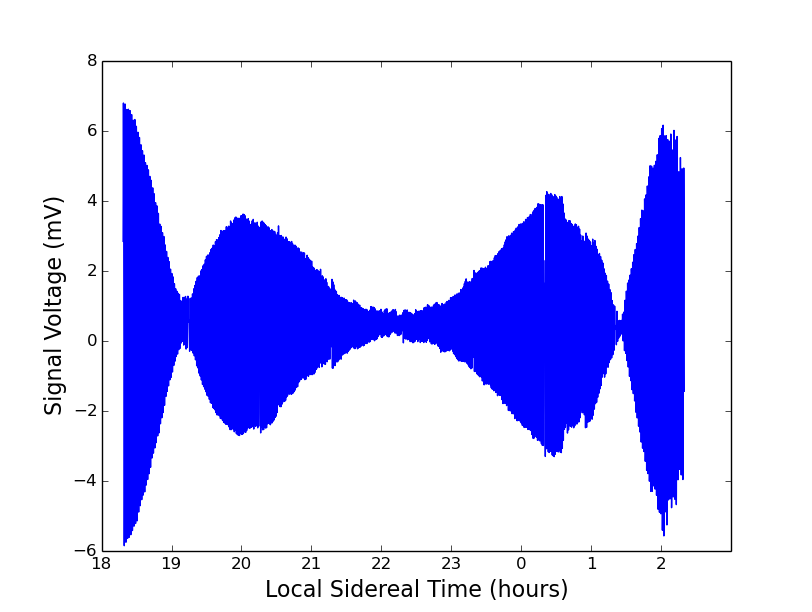
\includegraphics[width=0.78\linewidth]{figures/sun_old_all.png}
\caption{Benchmark (expected) Sun fringe pattern from 2007 data}
\label{fig:oldsun}
\end{figure}

\begin{figure}[h!]
\centering
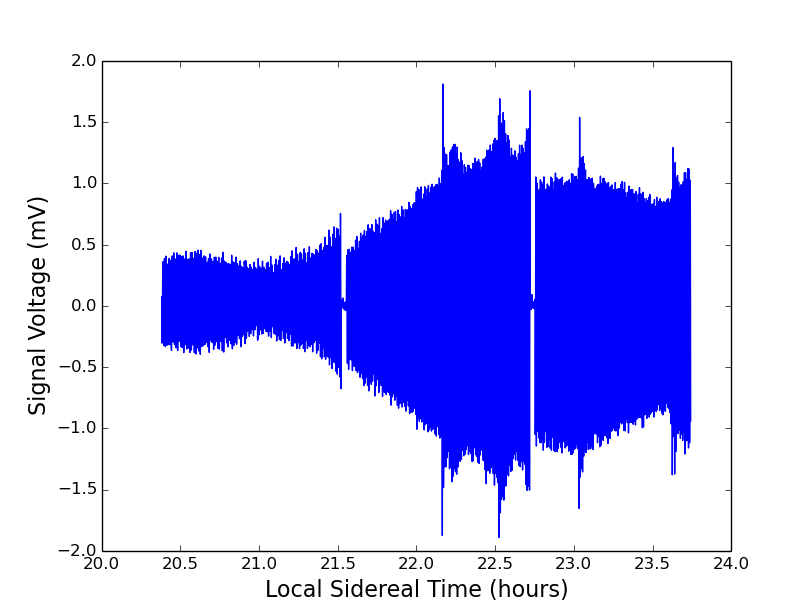
\includegraphics[width=0.78\linewidth]{figures/sun_new_all.png}
\caption{Collected Sun fringe pattern from March 12, 2015}
\label{fig:newsun}
\end{figure}

\begin{figure}[h!]
\centering
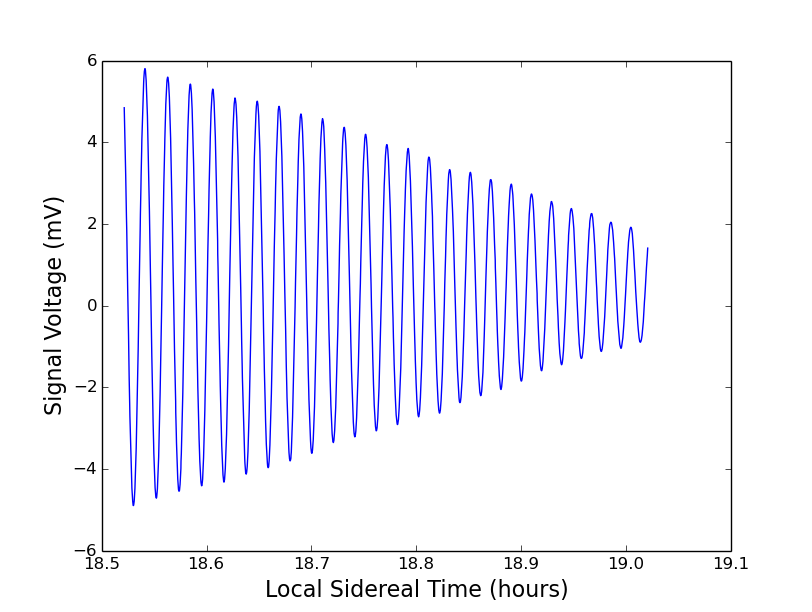
\includegraphics[width=0.74\linewidth]{figures/sun_old_small.png}
\caption{Benchmark (expected) Sun fringe pattern from 2007 data, zoomed in to half an hour showing a sinusoid}
\label{fig:oldsunsmall}
\end{figure}

\begin{figure}[h!]
\centering
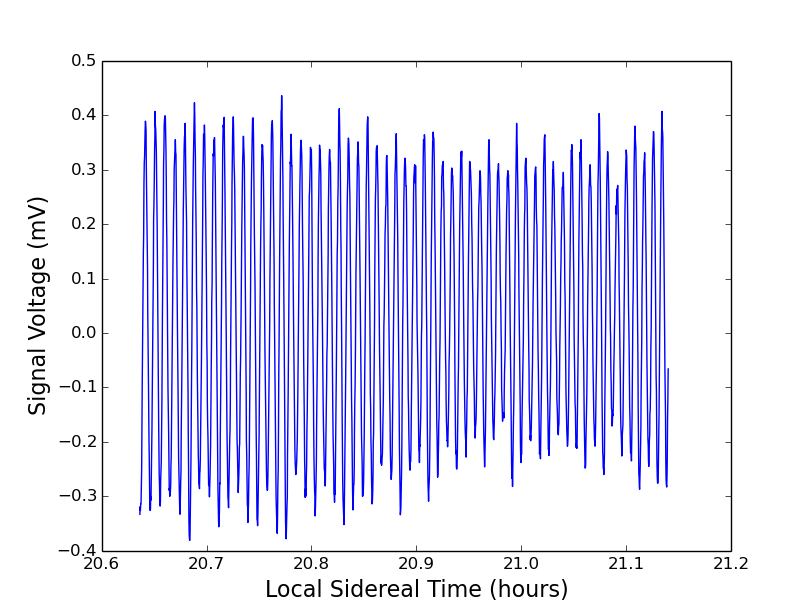
\includegraphics[width=0.74\linewidth]{figures/sun_new_small.png}
\caption{Collected Sun fringe pattern from March 12, 2015, zoomed in to half an hour showing a sinusoid}
\label{fig:newsunsmall}
\end{figure}

To measure the Sun's declination, least-squares fitting was done on the collected data.
From Equation 10 in the lab, ignoring any time-varying amplitude, the fringe amplitude should go as
\begin{equation}
F(h_s) = A \cos\left[ 2 \pi \left( \frac{B_y}{\lambda} \cos \delta \right) \sin h_s \right ] - B \sin \left[ 2 \pi \left( \frac{B_y}{\lambda} \cos \delta \right) \sin h_s \right ]
\end{equation}
since the interferometer used has an east-west baseline.
Here, $B_y$ is the baseline, which is 15.24 m, $\lambda$ is the measurement wavelength.
Because of the 1.7 GHz bandpass filter, the wavelength used comes from 12.3~GHz~-~1.7~GHz, giving a $\lambda$ of 2.83 cm.
Using linear least-squares fitting on the coefficients $A$ and $B$ while sweeping the declination resulted in Figure~\ref{fig:sunfit}.
This gives a measured declination value of 7.48\degree, though since cosine is an even function, this could be north or south of the celestial equator.
Results from the \texttt{isun} procedure give a declination of -3.22\degree, which agrees with the obtained result to within about 4\degree.

\begin{figure}
\centering
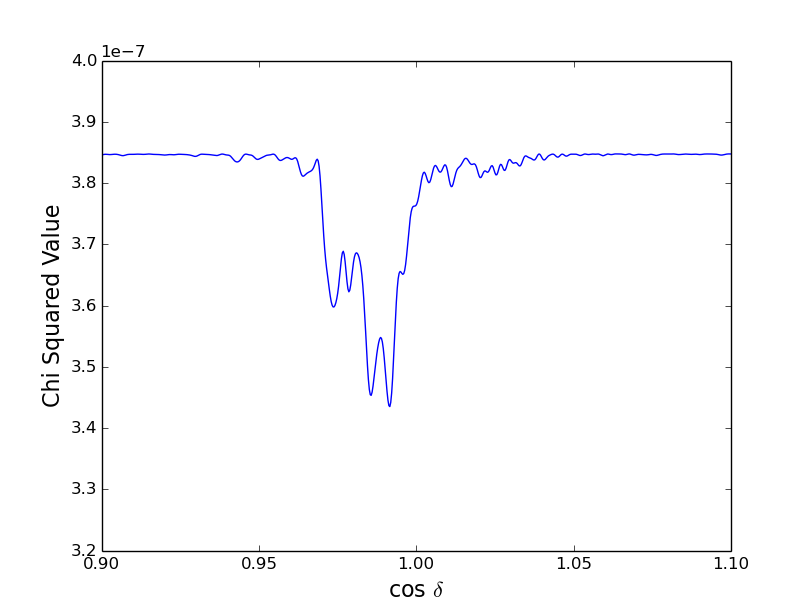
\includegraphics[width=\linewidth]{figures/sun_fit.png}
\caption{Linear least-squares fitting result on collected Sun data. The minimum occurs at a $\cos \delta$ of 0.9915.}
\label{fig:sunfit}
\end{figure}

To measure the fringe frequency the Fourier transform of the data was taken.
For the hour angles measured (-3.116 to 0.236 hours), the expected fringe frequencies can be found from
\begin{equation}
f_f = \left( \frac{B_y}{\lambda} \cos \delta \right) \cos h_s
\end{equation}
as taken from the lab manual Equation 12.
Expected fringe frequencies range from 26.8 mHz to 39.1 mHz.
This closely matches the actual DFT results, which are shown in Figure~\ref{fig:sundft}.

\begin{figure}
\centering
\includegraphics[width=\linewidth]{figures/sun_dft.eps}
\caption{DFT of the collected Sun fringe data}
\label{fig:sundft}
\end{figure}


\section{Point Source}

\subsection{Signal Quantization}

%% subfigure:
%\begin{figure}[h]
%    \centering
%    \begin{subfigure}[b]{0.44\textwidth}
%        \includegraphics[width=1.09\linewidth]{1v_hist}
%        \caption{Max voltage of 1 V}
%        \label{fig:1vhist}
%    \end{subfigure}
%    \quad
%    \begin{subfigure}[b]{0.46\textwidth}
%        \includegraphics[width=\linewidth]{100mv_hist}
%        \caption{Max voltage of 100 mV}
%        \label{fig:100mvhist}
%    \end{subfigure}
%    \caption{Voltage histograms showing quantization extent}
%\end{figure}
%
%% Figure:
%\begin{figure}
%\centering
%\includegraphics[width=0.75\linewidth]{raw_spectra}
%\caption{Spectral averages and medians with the HI line placed in either the LSB or USB.}
%\label{fig:rawspectra}
%\end{figure}

\enddocument
